\documentclass{article}

\usepackage{graphicx} 
\usepackage{hyperref}                         % Pacchetti
\usepackage[italian]{babel}
\graphicspath{ {./images/} }
\usepackage{fancyhdr}
\usepackage{imakeidx}


\makeindex[columns=1, title=Tavola dei contenuti, intoc]

\begin{document}
	
	
	\begin{titlepage}
		\begin{center}
			\huge\textbf{Montani WebSite}\\
			\Large\textbf{5 INB}\\
			\Large \textbf{Documento di Progettazione del Sito Web e Database}\\
			\vspace{4cm}
			\large Project Manager: \textbf{Boussoufa Yacine}\\
			\large Data: \textbf{08/02/2022}\\
			\large Versione: \textbf{0.1}\\
			\large ID WP: \textbf{Allegato D}\\
			\large ID Progetto: \textbf{Montani}\\
			
		\end{center}
	\end{titlepage}
	
	\clearpage
	
	\begin{tabular}{ |p{1cm}|p{4cm}|p{3cm}|p{2cm}|  }
		\hline
		\multicolumn{4}{|c|}{Cronologia delle revisioni} \\
		\hline
		ID& Cambiamenti &Data di creazione&Autore\\
		\hline
		001   & Creazione    &08/02/2022&   Camilletti Samuele\\
		\hline
	\end{tabular}
	
	\clearpage
	
	\tableofcontents
	\printindex	
	
   

    %_______________________________________________________________________________________________
    %ANALISI PROBLEMA	
	\section{\textbf{Introduzione al documento}}
	\flushleft
	\normalsize
	Il presente documento ha lo scopo di presentare la progettazione Front-End e Back-End del Sito Web sviluppato.
	\normalsize
	 \subsection{\textbf{Obiettivo}} 
	\flushleft
	\normalsize
	L'obiettivo del presente progetto è di realizzare un sito web per l'Istituto Tecnico Tecnologico Montani di Fermo. La scuola dispone già di un sito web, il quale non rispetta i requisiti grafici e funzionali definiti dal modello standard di siti web scolastici realizzato dal Team per la Trasformazione Digitale su richiesta del Ministero dell'Istruzione. Il progetto si basa sulla metodologia, gli strumenti e il design system di Designers Italia e a sua volta, contribuisce ad alimentare il design system della Pubblica Amministrazione mettendo a disposizione di tutte le amministrazioni componenti e pattern elaborati. Per ulteriori informazioni consultare \url{https://docs.italia.it/italia/designers-italia/design-scuole-docs/it/master/progetto-siti-web-delle-scuole.html}. Partendo dallo studio della realtà pre-esistente è stato necessario ridefinire le modalità di navigazione e di interfacciamento con l'utente nel sito web. Un'ulteriore campo di applicazione del sito web è l'accessibilità, ovvero la capacità del sistema informativo di erogare informazioni rispettando le linee guida sull’accessibilità degli strumenti informatici secondo quanto descritto nell’articolo 11 della legge n. 4/2004.

	\subsection{\textbf{Inquadramento}}
	Questo progetto mira a ridefinire il modello di fruizione dei servizi scolastici dell'Istituto T.T. Montani di Fermo attraverso il suo sito web.
	
	Il sito web è accessibile da qualsiasi device connesso ad internet, attraverso l'utilizzo di un browser web e digitando l'indirizzo istitutomontani.edu.it.\\
	Al caricamento della pagina verrà mostrata l'homepage, dalla quale si potrà scegliere il facilmente il servizio che l'utente sta cercando. 
	
	\subsubsection{\textbf{Piattaforme}}
	L’interfaccia sistema/utente è stata realizzata attraverso un sito web il quale utilizza il CSM Wordpress. WordPress è una piattaforma software di content management system (CMS) che, operando lato server in un database, consente la creazione di un sito Internet formato da contenuti testuali o multimediali, gestibili ed aggiornabili in maniera dinamica; facendo uso di codice HTML CSS e JavaScript. Wordpress mette a disposizione anche plugin e temi per la personalizzazione del sito web. Wordpress necessita di un database per la memorizzazione di tutte le informazioni relative al sito e un Web Server Apache. Per la mantenimento del web server e del relativo database viene utilizzato il servizio hosting Aruba. Il dominio (istitutomontani.edu.it) segue le normative relative agli indirizzi istituzionali.
	
	\subsubsection{\textbf{Progettazione del Sito Web}}
	La seguente progettazione illustra il lato Front-End e Back-end del sito e il rapporto dei soggetti coinvolti con esso.	
	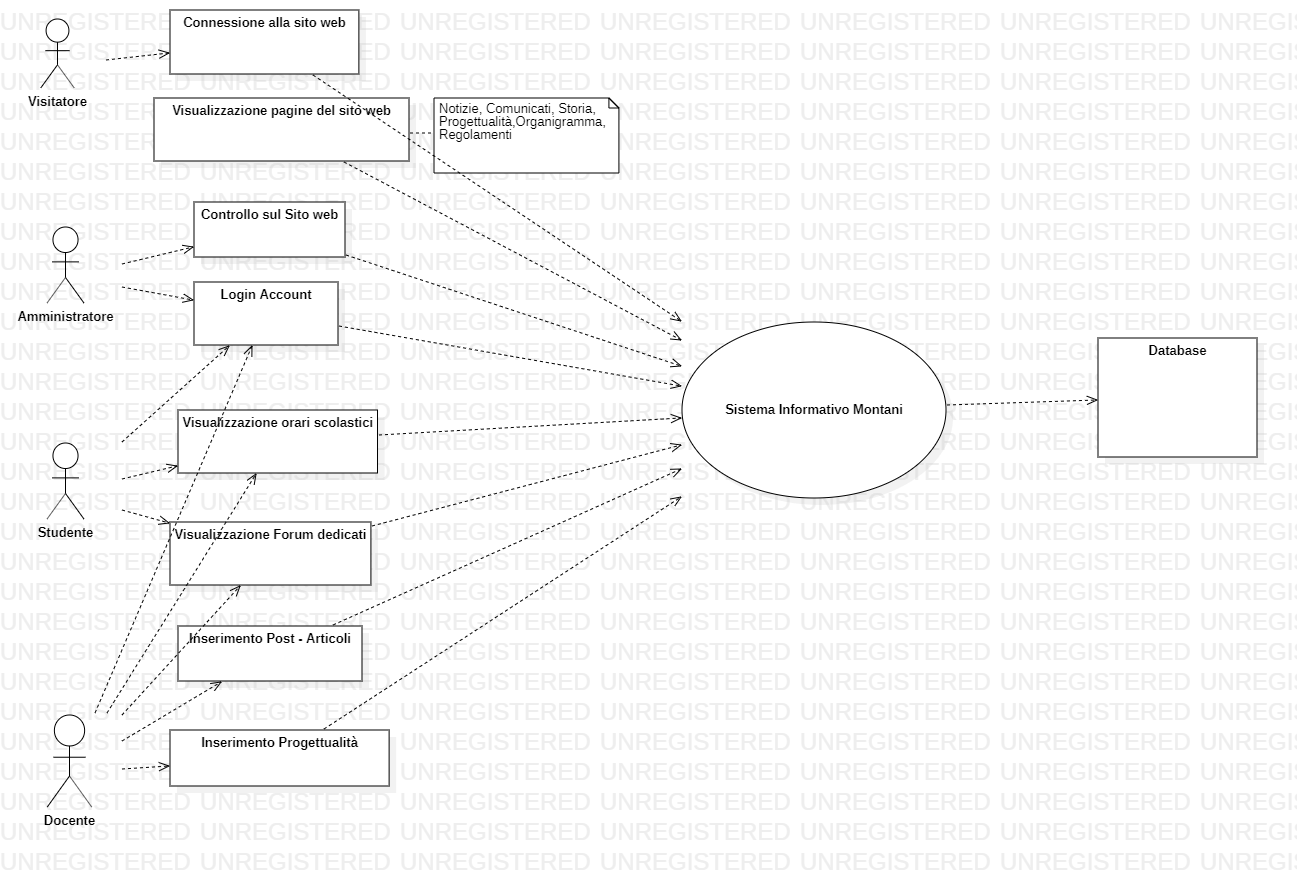
\includegraphics[scale=0.35]{UseCaseDiagram.png}
	
	\subsubsection{\textbf{Analisi Repository}}
	Per soddisfare i requisiti RF-005,RF-009 e RF-010 relativi al documento della Specifica dei Requisiti, è stato necessario progettare un ampliamento del Database preesistente di Wordpress al fine di consentire una gestione della repository efficiente nella medesima base di dati.
	In particolare, si intende gestire i dati relativi alla modulistica, libri di testo scolastici, progettualità e programmazioni scolastiche.
	Per modulistica scolastica si intende la raccolta di documenti utilizzabili dai soggetti che frequentano l'Istituto per richiedere o effettuare una procedura. I file sono caricati dalla Segreteria scolastica e sono messi a disposizione per tutti gli utenti coinvolti nel sistema. I moduli sono suddivisi per categoria di utente: alunni e famiglie, docenti, pubblico e personale ATA.
	La modulistica scolastica è definita da un link di download per un file .doc/.pdf caricato nell'archivio Wordpress, una data di caricamento, dimensione del file e il nome dell'autore.
	Per libri di testo scolastici si intende un file contenente le informazioni relative ai libri adottati dal docente, per una specifica classe dell'Istituto. I libri pubblicati dalla Segreteria scolastica sono visibili da tutti gli utenti del sistema; è da notare infatti che le classi prime non possedendo un indirizzo istituzionale non potrebbero visualizzare i testi scolastici senza aver effettuato l'accesso.
	I libri di testo scolastici sono suddivisi per anno scolastico e anno di corso(PRIME, SECONDE...) come nella versione precedente della repository e conterranno un link di download al relativo .pdf caricato nell'archivio. L'entità libro di testo conterrà inoltre una data di caricamento, la dimensione del file, il nome dell'autore e la rispettiva classe.
	I docenti e il committente hanno inoltre evidenziato la necessità di implementare un'ulteriore repository dedicata alle progettualità svolte nel corso degli anni.
	Un progetto si compone di un nome progetto, un obiettivo, una tipologia progetto (PCTO, Scuola e Territorio,...), una descrizione progetto, eventuali foto allegate, una data di realizzazione, il team di sviluppo e relativo file di progetto. I progetti sono inoltre caratterizzati da un Anno Scolastico, una classe e dalla relativa Articolazione.\\ 
	Per identificare univocamente un progetto si è scelto di utilizzare il nome progetto, in quanto non è opportuno, anche per motivi di diritto di autore, che esistano 2 progetti con lo stesso nome.
	Per associare le foto ad un progetto è stata definita un'entità foto la quale contiene le informazioni relative al percorso del file, ed è stato posto un limite ad un massimo di 3 foto per progetto.
	I progetti sono caricati dai docenti dell'Istituto e sono visibili a tutte le categorie di utenza, al fine di accrescere il lavoro svolto dagli studenti.\\
	Infine, è stato richiesto di implementare una repository dedicate alle programmazioni scolastiche svolte durante l'anno dalle singole classi dell'Istituto.
	Le programmazioni sono costituite da un link per il download di un file .pdf caricato nell'archivio, una data di caricamento, dimensione del file nome dell'autore, la classe, la materia e il relativo Anno Scolastico. Non sarà implementata un'entità materia, in quanto è impossibile fisicamente tenere traccia di tutte le materie e della loro evoluzione nel tempo.
	Le programmazioni, come per i progetti, possono essere caricati da utenti con permessi Docente.
	Le programmazioni possono essere visualizzate solo dagli utenti che hanno effettuato l'accesso al sistema.
	Un docente può caricare più progetti e più programmazioni. La segreteria può caricare più moduli e più libri di testo.
	Per identificare un account nel sistema si utilizza la progettazione fisica preesistente del database Wordpress, la quale memorizza gli account registrati in una tabella dedicata. 
	Come già specificato, i progetti, le programmazioni e i libri di testo saranno inoltre associati a una classe dell'Istituto. Una classe dell'Istituto sarà identificata da un'identificativo, una denominazione, un'anno di corso e l'anno scolastico corrente. Un anno scolastico identificherà univocamente i progetti, programmazioni e libri di testo nel tempo. La classe sarà inoltre associata ad un anno di corso (prime, seconde, terze, quarte, quinte). Su richiesta del committente la classe non sarà associata ad un anno scolastico, ma verrà riutilizzata nel corso degli anni, considerando che saranno i singoli documenti ad essere associati a un fattore temporale. 
	
	\subsubsection{\textbf{Individuazione delle entità}}

	\subsection{\textbf{Browser supportati}}

	\subsection{\textbf{Ottimizzazioni al motore di ricerca}}
	SEO, ....	
\clearpage
	
\section{\textbf{Ulteriori specifiche}}
Ulteriori specifiche, se necessarie, verranno aggiunte nelle prossime versioni del seguente documento.
\end{document}
	
    